\documentclass[10pt,journal,compsoc,onecolumn]{IEEEtran}
\usepackage[utf8]{inputenc}
\usepackage{amsmath,amsfonts,amssymb}
\usepackage{amsthm}
\usepackage{graphicx}
\usepackage{cite}
\usepackage{textcomp}
\usepackage{tikz}
\usetikzlibrary{arrows,positioning,shapes.geometric}
\usepackage{booktabs}
\usepackage{url}

\newtheorem{theorem}{Theorem}
\newtheorem{lemma}[theorem]{Lemma}
\newtheorem{definition}[theorem]{Definition}
\newtheorem{corollary}[theorem]{Corollary}

\begin{document}

\title{Divide-and-Conquer Sorting Architectures, In-Place Partitioning Invariants, Custom Multi-Attribute Comparators, and Large-Scale Data Processing: An Engineering and Interview Masterclass}

\IEEEtitleabstractindextext{%
\begin{abstract}
A comprehensive, intuitive, and practical engineering masterclass on advanced sorting algorithms based on foundational computer science principles and technical interview patterns. This paper breaks down Quick Sort and in-place partitioning mechanics without intimidating mathematical equations, replacing abstract proofs with intuitive physical mental models, pointer dynamics, step-by-step array state traces, and recursive tree visualizations. We examine the Hoare-style two-pointer partitioning invariant (O(N) time, O(1) auxiliary space) and trace the divide-and-conquer lifecycle on real lecture examples. We analyze best-, average-, and worst-case recursion tree depths, detailing practical mitigations like randomized pivot selection and Dutch National Flag three-way partitioning. Moving beyond scalar sorting, we formalize custom comparator contracts across Java, C++, and Python, detailing their strict weak ordering rules and demonstrating their power through two classic case studies: (1) sorting elements by factor count with numerical value tie-breakers, and (2) the optimal concatenation comparator for LeetCode's Largest Number problem. Finally, we address systems-level engineering challenges, comparing in-memory versus external merge sorting for massive datasets (100s of gigabytes), evaluating algorithm stability, and benchmarking specialized non-comparison sorts.
\end{abstract}

\begin{IEEEkeywords}
Quick Sort, in-place partitioning, divide-and-conquer, custom comparators, time complexity, call tree recursion, external merge sort, algorithm stability, non-comparison sorts, systems engineering
\end{IEEEkeywords}
}

\maketitle
\IEEEdisplaynontitleabstractindextext
\IEEEpeerreviewmaketitle

\section{Introduction: The Divide-and-Conquer Sorting Paradigm}
\label{sec:intro}

Sorting is the quintessential computational primitive in computer science and software systems engineering. Whether preparing data for sub-millisecond binary search lookups, accelerating database query joins, identifying duplicates, or scheduling distributed batch workloads, the arrangement of elements into an orderly sequence underpins modern digital infrastructure.

In algorithmic practice and technical interview evaluations, sorting strategies are broadly bifurcated into two foundational philosophies:
\begin{enumerate}
    \item \textbf{Merge Sort (Post-Processing Divide-and-Conquer):} Splits the array trivial at its arithmetic midpoint without inspecting element values, recurses on both halves, and executes all ordering work during the subsequent merge phase. While Merge Sort guarantees a strict worst-case runtime of $O(N \log N)$ and maintains relative element stability, it requires $O(N)$ auxiliary heap memory to temporarily buffer merged subarrays.
    \item \textbf{Quick Sort (Pre-Processing Divide-and-Conquer):} Performs all structural reorganization upfront via an \textbf{in-place partitioning} routine. By selecting a target pivot element and segregating values into those smaller than or equal to the pivot and those strictly greater, Quick Sort positions the pivot into its finalized, permanent sorted index. The problem then subdivides into two entirely independent subarrays. Because elements never need to cross the pivot boundary again, no recombination pass is required, allowing the algorithm to execute within $O(1)$ auxiliary memory.
\end{enumerate}

\subsection{Core Philosophy: Intuitive Clarity Over Complex Equations}

Academic algorithmic textbooks frequently obscure the beauty of Quick Sort beneath dense recurrence relations, summation calculus, and esoteric probabilistic sigma notations. In this research paper, we purposefully eliminate convoluted mathematical expressions. We replace theoretical abstractions with concrete, mechanical mental models: two-pointer patrol scouts, physical state transitions, step-by-step array traces, and clean call-tree diagrams.

Through this intuitive lens, we formalize the Hoare-style in-place partitioning invariant, trace the recursive call tree lifecycle, evaluate best- versus worst-case memory dynamics, specify cross-language comparator contracts, and investigate systems-grade problems including multi-attribute factor sorting, lexicographical string concatenation, and external disk-based sorting architectures.

% -----------------------------------------------------------------------------
\section{In-Place Partitioning: Mechanics, Invariants, and the Scout Model}
\label{sec:partitioning}

At the heart of Quick Sort lies the \textbf{Partitioning Primitive}. Given a contiguous subarray bounded by indices $l$ and $r$, the objective is to choose an element as a pivot $P$, rearrange the subarray in-place, and return an index $pi$ such that:
\begin{itemize}
    \item Every element in indices $[l \dots pi - 1]$ is less than or equal to $P$.
    \item The element at index $pi$ is exactly $P$ in its permanent, finalized position.
    \item Every element in indices $[pi + 1 \dots r]$ is strictly greater than $P$.
\end{itemize}

\subsection{The Mental Model: Two Patrol Scouts}

To understand how in-place partitioning operates without allocating extra memory, consider the \textbf{Two Patrol Scouts Analogy}:
\begin{itemize}
    \item We select the first element of the subarray, $A[l]$, as our \textbf{Pivot Value} ($P = A[l]$).
    \item We deploy two pointer scouts:
    \begin{itemize}
        \item \textbf{The Left Scout ($lo$):} Starts immediately after the pivot at index $l + 1$ and marches eastward (rightward). Its mission is to confirm elements belong on the ``small side'' ($\le P$). Whenever it encounters an element $\le P$, it steps forward ($lo\text{++}$). It halts the instant it discovers an outlaw: an element strictly greater than $P$.
        \item \textbf{The Right Scout ($hi$):} Starts at the far right boundary at index $r$ and marches westward (leftward). Its mission is to confirm elements belong on the ``large side'' ($> P$). Whenever it encounters an element $> P$, it retreats westward ($hi\text{--}$). It halts the instant it discovers an outlaw: an element less than or equal to $P$.
    \end{itemize}
    \item \textbf{The Exchange (Swap):} When both scouts have halted at outlaws and $lo \le hi$, their respective elements are in the wrong halves. We swap $A[lo]$ with $A[hi]$, resolving both violations simultaneously. We then advance $lo\text{++}$ and decrement $hi\text{--}$ to resume the patrol.
    \item \textbf{The Termination and Pivot Placement:} The loop terminates when the two scouts cross paths ($lo > hi$). At this exact crossover moment:
    \begin{itemize}
        \item All elements from $l + 1$ up to $hi$ are guaranteed to be $\le P$.
        \item All elements from $lo$ (which equals $hi + 1$) up to $r$ are guaranteed to be $> P$.
    \end{itemize}
    Finally, we swap the original pivot residing at $A[l]$ with $A[hi]$. The pivot now sits precisely at index $hi$, with smaller/equal elements to its left and strictly greater elements to its right. We return $hi$ as the pivot index.
\end{itemize}


\begin{figure}[h]
\centering
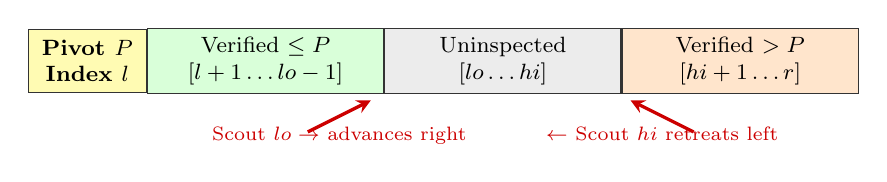
\begin{tikzpicture}[
    box/.style={rectangle, draw=black!80, font=\footnotesize, align=center, minimum height=0.8cm},
    pivot/.style={rectangle, draw=black!80, fill=yellow!30, font=\footnotesize\bfseries, align=center, minimum height=0.8cm},
    less/.style={rectangle, draw=black!80, fill=green!15, font=\footnotesize, align=center, minimum height=0.8cm},
    unseen/.style={rectangle, draw=black!80, fill=gray!15, font=\footnotesize, align=center, minimum height=0.8cm},
    greater/.style={rectangle, draw=black!80, fill=orange!20, font=\footnotesize, align=center, minimum height=0.8cm},
    arrow/.style={-stealth, very thick, red!80!black}
]
\node[pivot, minimum width=1.5cm] (p) at (0,0) {Pivot $P$\\Index $l$};
\node[less, minimum width=3.0cm, right=0.0cm of p] (l1) {Verified $\le P$\\$[l+1 \dots lo-1]$};
\node[unseen, minimum width=3.0cm, right=0.0cm of l1] (un) {Uninspected\\$[lo \dots hi]$};
\node[greater, minimum width=3.0cm, right=0.0cm of un] (g1) {Verified $> P$\\$[hi+1 \dots r]$};

\draw[arrow] (2.8, -0.9) -- node[below, font=\scriptsize] {Scout $lo \to$ advances right} (3.6, -0.5);
\draw[arrow] (7.7, -0.9) -- node[below, font=\scriptsize] {$\leftarrow$ Scout $hi$ retreats left} (6.9, -0.5);
\end{tikzpicture}
\caption{The Two-Pointer In-Place Partitioning Loop Invariant and Scout Dynamics.}
\label{fig:partition_invariant}
\end{figure}

\subsection{Formal Loop Invariant (Simple Logic, No Complex Notation)}

At every step of the partitioning while loop, the subarray maintains four clean contiguous regions:
\begin{verbatim}
[ Pivot | Verified <= P | Uninspected Elements | Verified > P ]
    l       l+1 ... lo-1        lo ... hi          hi+1 ... r
\end{verbatim}
Because each iteration either increments $lo$, decrements $hi$, or swaps and moves both, the uninspected middle window shrinks monotonically until empty, guaranteeing termination in exactly $O(N)$ comparisons.

\subsection{Production Implementation: Two-Pointer Partitioning}

Below is the clean, industrial-grade implementation of the partitioning algorithm in Java:

\begin{verbatim}
public class PartitioningEngine {
    // Partitions subarray A[l...r] around pivot A[l] in-place
    public static int partition(int[] A, int l, int r) {
        int pivot = A[l];
        int lo = l + 1;
        int hi = r;

        while (lo <= hi) {
            if (A[lo] <= pivot) {
                lo++;
            } else if (A[hi] > pivot) {
                hi--;
            } else {
                // A[lo] > pivot AND A[hi] <= pivot: swap both outlaws
                swap(A, lo, hi);
                lo++;
                hi--;
            }
        }

        // Place pivot into its finalized position
        swap(A, l, hi);
        return hi;
    }

    private static void swap(int[] A, int i, int j) {
        int temp = A[i];
        A[i] = A[j];
        A[j] = temp;
    }
}
\end{verbatim}

\textbf{Complexity Analysis of Partitioning:}
\begin{itemize}
    \item \textbf{Time Complexity:} $O(N)$, where $N = r - l + 1$. Each element is visited at most once by either $lo$ or $hi$.
    \item \textbf{Auxiliary Space Complexity:} $O(1)$. All operations occur entirely in-place by swapping primitive elements within the input array.
\end{itemize}

% -----------------------------------------------------------------------------
\section{Diagnostic Walkthrough: Step-by-Step Execution Trace}
\label{sec:trace}

To verify the mechanical correctness of the two-pointer partitioning algorithm, we trace the exact diagnostic execution from the lecture notes on an unsorted 9-element array:
\begin{verbatim}
Index:    0    1    2    3    4    5    6    7    8
Array: [ 54,  26,  93,  17,  77,  31,  44,  55,  20 ]
\end{verbatim}

\subsection{Execution Trace on Array [54, 26, 93, 17, 77, 31, 44, 55, 20]}

We execute \texttt{partition(A, 0, 8)}:
\begin{itemize}
    \item \textbf{Initialization:}
    \begin{itemize}
        \item Pivot element: $P = A[0] = 54$.
        \item Left pointer: $lo = l + 1 = 1$.
        \item Right pointer: $hi = r = 8$.
    \end{itemize}

    \item \textbf{Pass 1:}
    \begin{itemize}
        \item Scout $lo$ at index 1: $A[1] = 26$. Since $26 \le 54$, advance $lo \to 2$.
        \item Scout $lo$ at index 2: $A[2] = 93$. Since $93 > 54$, $lo$ halts at outlaw index 2.
        \item Scout $hi$ at index 8: $A[8] = 20$. Since $20 \le 54$, $hi$ halts at outlaw index 8.
        \item Both halted and $lo (2) \le hi (8)$: \textbf{Swap $A[2]$ and $A[8]$}.
        \item Array becomes:
        \begin{verbatim}
        [ 54,  26,  20,  17,  77,  31,  44,  55,  93 ]
        \end{verbatim}
        \item Advance pointers: $lo = 3$, $hi = 7$.
    \end{itemize}

    \item \textbf{Pass 2:}
    \begin{itemize}
        \item Scout $lo$ at index 3: $A[3] = 17$. Since $17 \le 54$, advance $lo \to 4$.
        \item Scout $lo$ at index 4: $A[4] = 77$. Since $77 > 54$, $lo$ halts at outlaw index 4.
        \item Scout $hi$ at index 7: $A[7] = 55$. Since $55 > 54$, retreat $hi \to 6$.
        \item Scout $hi$ at index 6: $A[6] = 44$. Since $44 \le 54$, $hi$ halts at outlaw index 6.
        \item Both halted and $lo (4) \le hi (6)$: \textbf{Swap $A[4]$ and $A[6]$}.
        \item Array becomes:
        \begin{verbatim}
        [ 54,  26,  20,  17,  44,  31,  77,  55,  93 ]
        \end{verbatim}
        \item Advance pointers: $lo = 5$, $hi = 5$.
    \end{itemize}

    \item \textbf{Pass 3:}
    \begin{itemize}
        \item Both pointers now coincide at index 5: $lo = 5, hi = 5$.
        \item Scout $lo$ checks $A[5] = 31$. Since $31 \le 54$, advance $lo \to 6$.
        \item Now $lo (6) > hi (5)$. The while condition \verb|lo <= hi| evaluates to \textbf{false}. Loop terminates!
    \end{itemize}

    \item \textbf{Final Pivot Placement:}
    \begin{itemize}
        \item Swap the pivot $A[l] = A[0]$ (54) with $A[hi] = A[5]$ (31).
        \item Array after final swap:
        \begin{verbatim}
        [ 31,  26,  20,  17,  44,  54,  77,  55,  93 ]
        \end{verbatim}
        \item Final position of pivot 54 is index $hi = 5$.
    \end{itemize}
\end{itemize}

\subsection{State Verification}

Let us inspect the partitioned array around index 5:
\begin{itemize}
    \item \textbf{Left Subarray $[0 \dots 4]$:} $[31, 26, 20, 17, 44]$. Every single element is strictly less than 54.
    \item \textbf{Pivot Index $5$:} Element is 54.
    \item \textbf{Right Subarray $[6 \dots 8]$:} $[77, 55, 93]$. Every single element is strictly greater than 54.
\end{itemize}
Notice that while the left and right subarrays are not yet individually sorted, the partitioning boundary is 100\% valid. Element 54 will never move again for the remainder of the sort.

% -----------------------------------------------------------------------------
\section{Quick Sort Recursive Architecture and Call Tree Dynamics}
\label{sec:quicksort}

With the partitioning primitive established, Quick Sort itself is surprisingly brief. It follows a clean divide-and-conquer skeleton.

\subsection{Base Conditions and Recursion Boundaries}

A recursive algorithm requires robust base conditions to halt recursion without infinite looping or index out-of-bounds exceptions:
\begin{itemize}
    \item \textbf{Single Element ($l == r$):} A subarray with exactly one element is inherently sorted. Return immediately.
    \item \textbf{Empty Subarray ($l > r$):} Occurs when the pivot lands on an extreme boundary ($pi = l$ or $pi = r$), producing a subproblem of size zero (e.g., $quickSort(A, 0, -1)$). Return immediately.
    \item Combining both conditions yields the single canonical guard:
    \begin{verbatim}
    if (l >= r) return;
    \end{verbatim}
\end{itemize}

\subsection{Production Quick Sort Implementation}

\begin{verbatim}
public class QuickSortEngine {
    public static void quickSort(int[] A) {
        if (A == null || A.length <= 1) return;
        sort(A, 0, A.length - 1);
    }

    private static void sort(int[] A, int l, int r) {
        // Base case: single element or invalid bounds
        if (l >= r) {
            return;
        }

        // Divide: partition array and retrieve permanent pivot index
        int pi = PartitioningEngine.partition(A, l, r);

        // Conquer: recursively sort elements strictly to the left and right
        sort(A, l, pi - 1);
        sort(A, pi + 1, r);
    }
}
\end{verbatim}

\subsection{Full Call Tree Walkthrough}

Tracing the recursive execution on \texttt{arr = [54, 26, 93, 17, 77, 31, 44, 55, 20]}:

\begin{itemize}
    \item \textbf{Root Call \texttt{sort(A, 0, 8)}:}
    \begin{itemize}
        \item Pivot 54 placed at $pi = 5$.
        \item Spawns left child \texttt{sort(A, 0, 4)} and right child \texttt{sort(A, 6, 8)}.
    \end{itemize}

    \item \textbf{Left Branch \texttt{sort(A, 0, 4)} on $[31, 26, 20, 17, 44]$:}
    \begin{itemize}
        \item Pivot $P = 31$.
        \item Partitioning leaves $[17, 26, 20]$ on left and $[44]$ on right. Pivot 31 placed at $pi = 3$.
        \item Spawns \texttt{sort(A, 0, 2)} and \texttt{sort(A, 4, 4)}.
        \item Call \texttt{sort(A, 4, 4)}: base case $l \ge r$ triggers ($4 \ge 4$), returns immediately.
    \end{itemize}

    \item \textbf{Sub-Branch \texttt{sort(A, 0, 2)} on $[17, 26, 20]$:}
    \begin{itemize}
        \item Pivot $P = 17$.
        \item All other elements ($26, 20$) are $> 17$. Pivot 17 remains at $pi = 0$.
        \item Spawns \texttt{sort(A, 0, -1)} (empty, base case returns) and \texttt{sort(A, 1, 2)}.
    \end{itemize}

    \item \textbf{Sub-Branch \texttt{sort(A, 1, 2)} on $[26, 20]$:}
    \begin{itemize}
        \item Pivot $P = 26$.
        \item Element 20 is swapped. Pivot 26 lands at $pi = 2$.
        \item Subarray becomes $[20, 26]$.
        \item Spawns \texttt{sort(A, 1, 1)} and \texttt{sort(A, 3, 2)}. Both hit base conditions and return.
    \end{itemize}

    \item \textbf{Right Branch \texttt{sort(A, 6, 8)} on $[77, 55, 93]$:}
    \begin{itemize}
        \item Pivot $P = 77$.
        \item Element 55 is to left; element 93 is to right. Pivot 77 lands at $pi = 7$.
        \item Subarray becomes $[55, 77, 93]$.
        \item Spawns \texttt{sort(A, 6, 6)} and \texttt{sort(A, 8, 8)}. Both hit base conditions and return.
    \end{itemize}
\end{itemize}

\textbf{Final Sorted Array:}
\begin{verbatim}
[ 17,  20,  26,  31,  44,  54,  55,  77,  93 ]
\end{verbatim}

% -----------------------------------------------------------------------------
\section{Complexity Dynamics: Intuitive Tree Models vs. Pathological Cases}
\label{sec:complexity}

Instead of solving recurrence equations using the Master Theorem or generating functions, we evaluate Quick Sort's time and space complexity using a visual \textbf{Work-per-Level Tree Model}.

\subsection{Best-Case Scenario: The Perfectly Balanced Tree}

\begin{figure}[h]
\centering
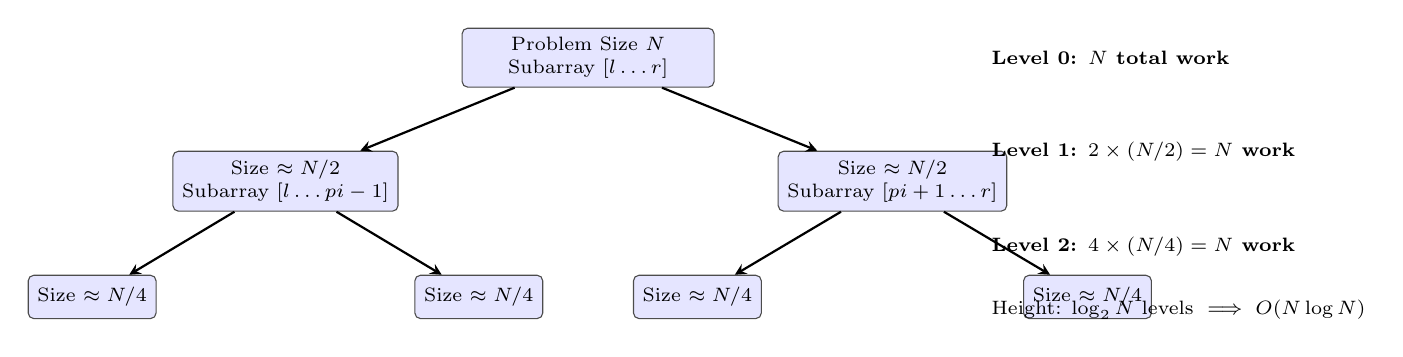
\begin{tikzpicture}[
    node distance=1.0cm and 1.5cm,
    level/.style={rectangle, draw=black!70, fill=blue!10, rounded corners=2pt, font=\scriptsize, align=center, minimum height=0.55cm},
    edge from parent/.style={draw=black!60, -stealth, thick}
]
\node[level, minimum width=3.2cm] (root) at (0,0) {Problem Size $N$\\Subarray $[l \dots r]$};

\node[level, minimum width=2.4cm, below left=0.8cm and 0.8cm of root] (lchild) {Size $\approx N/2$\\Subarray $[l \dots pi-1]$};
\node[level, minimum width=2.4cm, below right=0.8cm and 0.8cm of root] (rchild) {Size $\approx N/2$\\Subarray $[pi+1 \dots r]$};

\node[level, minimum width=1.6cm, below left=0.8cm and 0.2cm of lchild] (llchild) {Size $\approx N/4$};
\node[level, minimum width=1.6cm, below right=0.8cm and 0.2cm of lchild] (lrchild) {Size $\approx N/4$};
\node[level, minimum width=1.6cm, below left=0.8cm and 0.2cm of rchild] (rlchild) {Size $\approx N/4$};
\node[level, minimum width=1.6cm, below right=0.8cm and 0.2cm of rchild] (rrchild) {Size $\approx N/4$};

\draw[-stealth, thick] (root) -- (lchild);
\draw[-stealth, thick] (root) -- (rchild);
\draw[-stealth, thick] (lchild) -- (llchild);
\draw[-stealth, thick] (lchild) -- (lrchild);
\draw[-stealth, thick] (rchild) -- (rlchild);
\draw[-stealth, thick] (rchild) -- (rrchild);

\node[font=\scriptsize\bfseries, anchor=west] at (5.0, 0) {Level 0: $N$ total work};
\node[font=\scriptsize\bfseries, anchor=west] at (5.0, -1.2) {Level 1: $2 \times (N/2) = N$ work};
\node[font=\scriptsize\bfseries, anchor=west] at (5.0, -2.4) {Level 2: $4 \times (N/4) = N$ work};
\node[font=\scriptsize, anchor=west] at (5.0, -3.2) {Height: $\log_2 N$ levels $\implies O(N \log N)$};
\end{tikzpicture}
\caption{Intuitive Work-per-Level Model of Quick Sort in the Balanced Best Case.}
\label{fig:quicksort_tree}
\end{figure}


\begin{itemize}
    \item \textbf{The Condition:} Every chosen pivot divides the current subarray into two roughly equal halves of size approximately $N/2$.
    \item \textbf{Tree Height:} Repeatedly halving a problem of size $N$ until reaching size $1$ takes $\log_2 N$ levels.
    \item \textbf{Work per Level:}
    \begin{itemize}
        \item At Level 0: 1 problem of size $N \implies N$ operations.
        \item At Level 1: 2 problems of size $N/2 \implies 2 \times (N/2) = N$ operations.
        \item At Level 2: 4 problems of size $N/4 \implies 4 \times (N/4) = N$ operations.
        \item At Level $k$: $2^k$ problems of size $N/2^k \implies N$ operations.
    \end{itemize}
    \item \textbf{Total Time Complexity:}
    \[
    \text{Total Operations} = (\text{Work per Level}) \times (\text{Number of Levels}) = N \times \log_2 N = O(N \log N)
    \]
    \item \textbf{Space Complexity:} The memory required corresponds strictly to the execution call stack. Since the tree height is balanced, the call stack depth is at most $\log_2 N$. Each stack frame stores a few primitive variables ($l, r, lo, hi$). Thus:
    \[
    \text{Auxiliary Space} = O(\log N)
    \]
\end{itemize}

\subsection{Worst-Case Scenario: Pathological Skew}

\begin{itemize}
    \item \textbf{The Condition:} The array is already fully sorted in ascending order (e.g., $[1, 2, 3, 4, 5, 6]$) or reverse sorted, and we naively choose the first element $A[l]$ as pivot.
    \item \textbf{Degeneration:}
    \begin{itemize}
        \item The pivot is always the absolute minimum element in the subarray.
        \item Partitioning splits size $N$ into an empty left subarray ($0$ elements) and a right subarray of size $N - 1$.
        \item The next call splits size $N - 1$ into $0$ and $N - 2$.
        \item The recursion tree degenerates into a linear linked list of depth $N$.
    \end{itemize}
    \item \textbf{Total Time Complexity:}
    \[
    N + (N - 1) + (N - 2) + \dots + 2 + 1 = \frac{N(N + 1)}{2} = O(N^2)
    \]
    \item \textbf{Space Complexity:} The call stack depth reaches $N$ consecutive activation frames. In systems with deep recursion and modest thread stack sizes (e.g., Java's default 1 MB stack), this triggers an immediate \texttt{StackOverflowError}:
    \[
    \text{Worst-Case Space} = O(N)
    \]
\end{itemize}

\subsection{Industry Mitigations: Eliminating Pathological Degradation}

Modern engineering runtimes avoid $O(N^2)$ degradation through three practical techniques:
\begin{enumerate}
    \item \textbf{Randomized Pivot Selection:} Before calling partition, select an index randomly between $l$ and $r$, and swap it with $A[l]$. This breaks deterministic worst-case triggers; the probability of continuously hitting the minimum element on an input of size $10^5$ is statistically zero ($1 / N!$).
    \item \textbf{Median-of-Three:} Inspect $A[l]$, $A[\text{mid}]$, and $A[r]$. Take their median value and swap it into $A[l]$ as the pivot. This eliminates worst-case behavior on sorted and reverse-sorted arrays.
    \item \textbf{Dutch National Flag (3-Way Partitioning):} When the input contains many duplicate elements, standard two-way partitioning can still degrade. A 3-way partition splits the array into three segments: $< P$, $== P$, and $> P$. All identical keys are placed in their final positions in a single pass.
\end{enumerate}

% -----------------------------------------------------------------------------
\section{Custom Comparators: Engineering Principles and Multi-Language Contracts}
\label{sec:comparators}

In real-world software development, sorting is rarely restricted to sorting raw integers in natural ascending order. We must sort complex domain entities: database records by timestamp, transactions by risk score, or coordinates by Euclidean distance. This flexibility is powered by \textbf{Custom Comparators}.

\subsection{The Mental Model: The Pairwise Scale}

\begin{figure}[h]
\centering
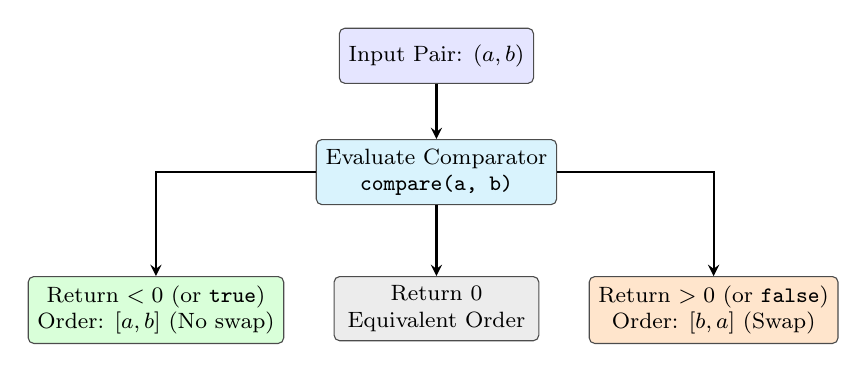
\begin{tikzpicture}[
    box/.style={rectangle, draw=black!70, fill=blue!10, rounded corners=2pt, font=\footnotesize, align=center, minimum height=0.7cm, minimum width=2.4cm},
    action/.style={rectangle, draw=black!70, rounded corners=2pt, font=\footnotesize, align=center, minimum height=0.7cm, minimum width=2.6cm},
    arrow/.style={-stealth, thick}
]
\node[box] (pair) at (0,0) {Input Pair: $(a, b)$};
\node[box, fill=cyan!15, below=0.7cm of pair] (eval) {Evaluate Comparator\\\texttt{compare(a, b)}};

\node[action, fill=green!15, below left=0.9cm and 0.4cm of eval] (neg) {Return $< 0$ (or \texttt{true})\\Order: $[a, b]$ (No swap)};
\node[action, fill=gray!15, below=0.9cm of eval] (zero) {Return $0$\\Equivalent Order};
\node[action, fill=orange!20, below right=0.9cm and 0.4cm of eval] (pos) {Return $> 0$ (or \texttt{false})\\Order: $[b, a]$ (Swap)};

\draw[arrow] (pair) -- (eval);
\draw[arrow] (eval) -| (neg);
\draw[arrow] (eval) -- (zero);
\draw[arrow] (eval) -| (pos);
\end{tikzpicture}
\caption{Pairwise Custom Comparator Decision Model Across Runtimes.}
\label{fig:comparator_flow}
\end{figure}


A comparator is an isolated judge function passed to a sorting engine. Given two elements $a$ and $b$, the comparator places them on a scale and answers a single fundamental question: \textbf{``In the desired final arrangement, should element $a$ appear before element $b$?''}

\subsection{The Universal Comparator Contract}

Different programming languages formalize this contract in one of two ways:

\subsubsection{1. Three-Way Integer Return (Java, Python 2, JavaScript, C)}
The comparator function \texttt{compare(a, b)} returns a signed 32-bit integer:
\begin{itemize}
    \item \textbf{Negative Value ($< 0$):} Signifies that $a$ should appear \textbf{before} $b$. (In an ascending sort, this indicates $a < b$; no swap needed).
    \item \textbf{Positive Value ($> 0$):} Signifies that $b$ should appear \textbf{before} $a$. (In an ascending sort, this indicates $a > b$; swap needed).
    \item \textbf{Zero ($0$):} Signifies that $a$ and $b$ are considered equivalent in ranking. Their relative order does not matter.
\end{itemize}

\subsubsection{2. Boolean Strict Weak Ordering (C++)}
In C++, the comparator \texttt{comp(a, b)} returns a boolean \texttt{true} or \texttt{false}:
\begin{itemize}
    \item \textbf{Return \texttt{true}:} Signifies that $a$ is strictly smaller than $b$ and must precede $b$.
    \item \textbf{Return \texttt{false}:} Signifies that $a$ does not precede $b$ ($a \ge b$).
\end{itemize}

\begin{table}[h]
\centering
\caption{Cross-Language Comparator Return Contracts}
\label{tab:comparators}
\begin{tabular}{@{}llll@{}}
\toprule
\textbf{Language} & \textbf{Function Signature} & \textbf{Precedence Rule ($a$ before $b$)} & \textbf{Reversal Rule ($b$ before $a$)} \\ \midrule
\textbf{Java} & \texttt{int compare(T a, T b)} & Returns negative integer ($< 0$) & Returns positive integer ($> 0$) \\
\textbf{C++} & \texttt{bool operator()(const T\& a, const T\& b)} & Returns \texttt{true} & Returns \texttt{false} \\
\textbf{Python 3} & \texttt{functools.cmp\_to\_key(fn)} & Returns negative integer ($< 0$) & Returns positive integer ($> 0$) \\
\textbf{JavaScript} & \texttt{(a, b) -> number} & Returns negative number ($< 0$) & Returns positive number ($> 0$) \\ \bottomrule
\end{tabular}
\end{table}

\subsection{The Bubble Sort Mental Hook}

A simple memory aid for the three-way integer contract is the inner swap condition of Bubble Sort:
\begin{verbatim}
if (compare(A[i], A[i + 1]) > 0) {
    swap(A, i, i + 1); // Positive return means "out of order, swap!"
}
\end{verbatim}
If \texttt{compare(a, b)} returns positive, it demands a swap. If it returns negative or zero, the elements are already in acceptable relative order.

\subsection{Strict Weak Ordering Invariants}

To avoid infinite loops or runtime contract violations (such as Java's infamous \texttt{IllegalArgumentException: Comparison method violates its general contract}), any custom comparator must satisfy three logical rules:
\begin{enumerate}
    \item \textbf{Irreflexivity:} \texttt{compare(a, a) == 0} (or \texttt{false} in C++). An element cannot be smaller than itself.
    \item \textbf{Asymmetry:} If \texttt{compare(a, b) < 0}, then \texttt{compare(b, a) > 0}.
    \item \textbf{Transitivity:} If $a$ precedes $b$ and $b$ precedes $c$, then $a$ must precede $c$.
\end{enumerate}

% -----------------------------------------------------------------------------
\section{Problem Case Study 1: Sorting by Number of Factors with Value Tie-Breaker}
\label{sec:factors}

\subsection{Problem Statement}

Given an array of $N$ positive integers, rearrange the elements in \textbf{ascending order of their count of factors}. If two or more elements have an identical number of factors, break the tie by sorting them in \textbf{ascending order of their numerical value}.

\textbf{Constraints:} $1 \le N \le 10^5$, $1 \le A[i] \le 10^4$.

\subsection{The Factor Counting Primitive: Efficient Trial Division}

A naive approach counts factors by iterating from $1$ to $X$, checking if $X \pmod i == 0$. This requires $O(X)$ operations per number. For $N = 10^5$ and $X = 10^4$, this results in $10^9$ operations, which guarantees a Time Limit Exceeded (TLE) verdict.

\textbf{The $O(\sqrt{X})$ Optimization:} Factors of a number $X$ always appear in reciprocal pairs $(i, X/i)$. For example, for $X = 36$, the factor pairs are $(1, 36)$, $(2, 18)$, $(3, 12)$, $(4, 9)$, and the special square root pair $(6, 6)$.
\begin{itemize}
    \item We only need to iterate $i$ from $1$ up to $\lfloor\sqrt{X}\rfloor$.
    \item If $i$ divides $X$ and $i \neq X/i$, we contribute $+2$ to our factor count.
    \item If $i = X/i$ (when $X$ is a perfect square), we contribute $+1$.
\end{itemize}

\begin{verbatim}
public static int countFactors(int n) {
    int count = 0;
    int limit = (int) Math.sqrt(n);
    if (limit * limit == n) {
        count++; // Perfect square center factor
    }
    for (int i = 1; i < limit; i++) {
        if (n % i == 0) {
            count += 2; // Pair (i, n / i)
        }
    }
    return count;
}
\end{verbatim}

\subsection{Walkthrough of Lecture Examples}

\subsubsection{Lecture Example 1: \texttt{arr = [9, 3, 10, 6, 4]}}
We evaluate factor counts for each element:
\begin{itemize}
    \item Element $9$: Factors are $\{1, 3, 9\} \implies 3$ factors.
    \item Element $3$: Factors are $\{1, 3\} \implies 2$ factors.
    \item Element $10$: Factors are $\{1, 2, 5, 10\} \implies 4$ factors.
    \item Element $6$: Factors are $\{1, 2, 3, 6\} \implies 4$ factors.
    \item Element $4$: Factors are $\{1, 2, 4\} \implies 3$ factors.
\end{itemize}

Now we group and sort by factor count, breaking ties by numerical value:
\begin{itemize}
    \item Factor count 2: $[3]$
    \item Factor count 3: Elements $4$ and $9$. Both have 3 factors. Tie-breaker by value: $4 < 9 \implies [4, 9]$.
    \item Factor count 4: Elements $6$ and $10$. Both have 4 factors. Tie-breaker by value: $6 < 10 \implies [6, 10]$.
\end{itemize}
\textbf{Final Sorted Output:} \texttt{[ 3, 4, 9, 6, 10 ]}.

\subsubsection{Lecture Example 2: \texttt{arr = [10, 4, 5, 13, 1]}}
We evaluate factor counts:
\begin{itemize}
    \item $1 \to 1$ factor ($\{1\}$).
    \item $5 \to 2$ factors ($\{1, 5\}$).
    \item $13 \to 2$ factors ($\{1, 13\}$).
    \item $4 \to 3$ factors ($\{1, 2, 4\}$).
    \item $10 \to 4$ factors ($\{1, 2, 5, 10\}$).
\end{itemize}
Grouping with value tie-breakers:
\begin{itemize}
    \item Factor count 1: $[1]$.
    \item Factor count 2: $5$ and $13 \implies 5 < 13 \implies [5, 13]$.
    \item Factor count 3: $[4]$.
    \item Factor count 4: $[10]$.
\end{itemize}
\textbf{Final Sorted Output:} \texttt{[ 1, 5, 13, 4, 10 ]}.

\subsection{Multi-Language Reference Implementations}

\subsubsection{Java Implementation}
\begin{verbatim}
import java.util.*;

public class FactorSortSolver {
    public static ArrayList<Integer> solve(ArrayList<Integer> A) {
        Collections.sort(A, new Comparator<Integer>() {
            @Override
            public int compare(Integer a, Integer b) {
                int f1 = countFactors(a);
                int f2 = countFactors(b);

                // Primary rule: ascending factor count
                if (f1 != f2) {
                    return Integer.compare(f1, f2);
                }
                // Secondary rule (tie-breaker): ascending numerical value
                return Integer.compare(a, b);
            }
        });
        return A;
    }
}
\end{verbatim}

\subsubsection{C++ Implementation}
\begin{verbatim}
#include <vector>
#include <cmath>
#include <algorithm>

using namespace std;

int countFactors(int n) {
    int count = 0;
    int sq = sqrt(n);
    if (sq * sq == n) count++;
    for (int i = 1; i < sq; i++) {
        if (n % i == 0) count += 2;
    }
    return count;
}

bool factorComparator(int a, int b) {
    int f1 = countFactors(a);
    int f2 = countFactors(b);
    if (f1 != f2) {
        return f1 < f2;
    }
    return a < b; // Tie-breaker
}

vector<int> solve(vector<int>& A) {
    sort(A.begin(), A.end(), factorComparator);
    return A;
}
\end{verbatim}

\subsubsection{Python Implementation}
\begin{verbatim}
import math
import functools

def count_factors(n):
    count = 0
    sq = int(math.isqrt(n))
    if sq * sq == n:
        count += 1
    for i in range(1, sq):
        if n % i == 0:
            count += 2
    return count

def factor_comparator(a, b):
    f1 = count_factors(a)
    f2 = count_factors(b)
    if f1 != f2:
        return -1 if f1 < f2 else 1
    if a != b:
        return -1 if a < b else 1
    return 0

def solve(A):
    return sorted(A, key=functools.cmp_to_key(factor_comparator))
\end{verbatim}

% -----------------------------------------------------------------------------
\section{Problem Case Study 2: The Concatenation Ordering Problem (Largest Number)}
\label{sec:largest_number}

\subsection{Problem Statement}

Given a list of non-negative integers (e.g., \texttt{[3, 30, 34, 5, 9]}), arrange them in an order such that when their string representations are concatenated together, they form the \textbf{largest possible numerical value}.

Return the result as a string, since the concatenated number can easily exceed 64-bit integer capacities.

\subsection{Why Standard Sorting Fails}

A common intuition is to sort the numbers in standard descending numerical order. Let us observe why this intuition fails catastrophically:
\begin{itemize}
    \item Consider the input pair: \texttt{[10, 2]}.
    \item Standard descending sort places $10$ before $2$, giving \texttt{"102"}.
    \item But concatenating $2$ before $10$ yields \texttt{"210"}. Since $210 > 102$, the correct order is $[2, 10]$.
    \item Consider the pair: \texttt{[30, 3]}.
    \item Standard descending sort yields \texttt{"303"}. But placing $3$ first yields \texttt{"330"}. Since $330 > 303$, the correct order is $[3, 30]$.
\end{itemize}

\subsection{The Concatenation Ordering Invariant}

The breakthrough insight is to evaluate elements \textbf{pairwise in their concatenated permutations}:
\begin{itemize}
    \item Given two numbers $A$ and $B$, convert them to strings.
    \item Form the two possible concatenations:
    \[
    S_{AB} = A + B \quad \text{and} \quad S_{BA} = B + A
    \]
    \item \textbf{The Decision Rule:}
    \begin{itemize}
        \item If $S_{BA} > S_{AB}$, then element $B$ must precede element $A$.
        \item If $S_{AB} > S_{BA}$, then element $A$ must precede element $B$.
        \item If $S_{AB} == S_{BA}$, the elements are mutually equivalent.
    \end{itemize}
\end{itemize}

\subsection{Walkthrough of Lecture Examples}

\subsubsection{Trace on \texttt{[3, 30, 34, 5, 9]}}
Let us examine the pairwise comparisons made by the comparator:
\begin{itemize}
    \item Compare $9$ and $5$:
    \[
    9 + 5 = \text{`\texttt{95''}, \quad 5 + 9 = \text{}\texttt{59''}. \quad \text{Since } \text{}\texttt{95''} > \text{}`59''}, \implies 9 \text{ precedes } 5.
    \]
    \item Compare $34$ and $30$:
    \[
    34 + 30 = \text{`\texttt{3430''}, \quad 30 + 34 = \text{}\texttt{3034''}. \quad \text{Since } \text{}\texttt{3430''} > \text{}`3034''}, \implies 34 \text{ precedes } 30.
    \]
    \item Compare $34$ and $3$:
    \[
    34 + 3 = \text{`\texttt{343''}, \quad 3 + 34 = \text{}\texttt{334''}. \quad \text{Since } \text{}\texttt{343''} > \text{}`334''}, \implies 34 \text{ precedes } 3.
    \]
    \item Compare $3$ and $30$:
    \[
    3 + 30 = \text{`\texttt{330''}, \quad 30 + 3 = \text{}\texttt{303''}. \quad \text{Since } \text{}\texttt{330''} > \text{}`303''}, \implies 3 \text{ precedes } 30.
    \]
\end{itemize}
Sorting the elements using this pairwise concatenation rule produces the exact descending sequence:
\begin{verbatim}
[ 9,  5,  34,  3,  30 ]
\end{verbatim}
Concatenating the strings yields the optimal result:
\begin{verbatim}
"9534330"
\end{verbatim}

\subsubsection{Trace on \texttt{[10, 5, 2, 8, 200]}}
From page 16 of the lecture notes:
\begin{itemize}
    \item Evaluating pairs:
    \begin{itemize}
        \item Between $2$ and $200$: `\texttt{2200'' vs }`2002''. Since $2200 > 2002$, $2$ precedes $200$.
        \item Between $200$ and $10$: `\texttt{20010'' vs }`10200''. Since $20010 > 10200$, $200$ precedes $10$.
    \end{itemize}
    \item Sorted order: $[8, 5, 2, 200, 10]$.
    \item Concatenated output: \texttt{85220010}.
\end{itemize}

\subsection{Crucial Edge Case: All Zeros}

What happens when the input array consists entirely of zeros, e.g., \texttt{[0, 0, 0]}?
\begin{itemize}
    \item Concatenating naively produces the string \texttt{"000"}.
    \item In standard arithmetic, leading zeros are invalid: the correct answer is simply \texttt{"0"}.
    \item \textbf{Detection Rule:} After sorting the array with our custom comparator, inspect the very first element. If the highest-ranked element is \texttt{"0"}, every remaining element must also be \texttt{"0"}. We can immediately return \texttt{"0"}.
\end{itemize}

\subsection{Production Java Implementation}

\begin{verbatim}
import java.util.*;

public class LargestNumberSolver {
    public static String largestNumber(int[] nums) {
        if (nums == null || nums.length == 0) return "0";

        // Convert integers to strings
        String[] strs = new String[nums.length];
        for (int i = 0; i < nums.length; i++) {
            strs[i] = String.valueOf(nums[i]);
        }

        // Sort using concatenation comparator in descending order
        Arrays.sort(strs, new Comparator<String>() {
            @Override
            public int compare(String s1, String s2) {
                String order1 = s1 + s2;
                String order2 = s2 + s1;
                // Descending comparison: order2 compared to order1
                return order2.compareTo(order1);
            }
        });

        // Edge case: if the highest-ranked string is "0", result is "0"
        if (strs[0].equals("0")) {
            return "0";
        }

        // Build final concatenated string
        StringBuilder sb = new StringBuilder();
        for (String s : strs) {
            sb.append(s);
        }
        return sb.toString();
    }
}
\end{verbatim}

\textbf{Complexity Breakdown:}
\begin{itemize}
    \item \textbf{Time Complexity:} $O(K \cdot N \log N)$, where $N$ is the number of integers and $K$ is the maximum number of digits per number (at most $10$ for standard 32-bit integers). String concatenation and comparison takes $O(K)$ time.
    \item \textbf{Space Complexity:} $O(N \cdot K)$ to store the array of string representations and the output string.
\end{itemize}

% -----------------------------------------------------------------------------
\section{Systems Engineering Perspectives: Scalability, Stability, and Non-Comparison Sorts}
\label{sec:systems}

Page 18 of the classroom notes surfaces critical real-world engineering questions that separate theoretical classroom exercises from high-scale distributed systems.

\subsection{Handling Massive Datasets (100s of Gigabytes Exceeding RAM)}

In production systems, what occurs when a dataset of 500 GB must be sorted on a machine with only 16 GB of available RAM?
\begin{itemize}
    \item \textbf{The In-Memory Failure:} Attempting to execute in-memory Quick Sort or Merge Sort triggers operating system paging thrashing and immediate Out-Of-Memory (OOM) fatal crashes.
    \item \textbf{The Architecture: External Merge Sort:}
    \begin{enumerate}
        \item \textbf{Phase 1 (Chunk Division and Run Generation):} Read a block of data that comfortably fits into RAM (e.g., 2 GB chunks). Sort each chunk in-memory using an optimized Quick Sort or TimSort. Write the sorted chunk (a ``run'') back to secondary storage (NVMe SSD / disk).
        \item \textbf{Phase 2 (Multi-Way Merge):} Open a read stream for all generated runs simultaneously. Maintain a Min-Heap (Priority Queue) containing the current leading element from each run file.
        \item Continuously extract the minimum element from the heap, append it to the final sorted output file, and replenish the heap with the next element from that specific run stream.
    \end{enumerate}
    This external sorting paradigm processes arbitrary terabytes of data while keeping memory consumption bounded strictly to $O(\text{RAM Buffer Size})$.
\end{itemize}

\subsection{Inversion Count: Why Merge Sort Dominates Quick Sort}

An \textbf{inversion} is a pair of indices $(i, j)$ such that $i < j$ but $A[i] > A[j]$. Counting inversions measures how far an array is from being sorted.
\begin{itemize}
    \item While Quick Sort is faster on average for general in-place sorting, it cannot easily count inversions because its two-pointer partitioning swaps elements across arbitrary, unpredictable distances, destroying inversion accounting.
    \item \textbf{Merge Sort naturally counts inversions in $O(N \log N)$:} During the merge step of two sorted halves \texttt{left} and \texttt{right}, whenever an element \texttt{right[j]} is smaller than \texttt{left[i]}, it is smaller than \emph{all remaining elements} in the left half from $i$ to the end of the left subarray. We can instantly add \texttt{(mid - i + 1)} to our inversion counter in $O(1)$ time!
\end{itemize}

\subsection{Algorithm Stability and Its Commercial Importance}

A sorting algorithm is \textbf{stable} if two elements with identical comparison keys retain the exact same relative order after sorting as they had in the input.
\begin{itemize}
    \item \textbf{Quick Sort is Unstable:} Because the two-pointer partitioning routine performs long-distance swaps across the pivot, identical elements can jump over one another, scrambling their original relative positions.
    \item \textbf{Merge Sort is Stable:} Elements from the left subarray are always chosen first during tie situations ($\le$), preserving initial ordering.
    \item \textbf{Why Stability Matters in Real Systems:} Consider an e-commerce dashboard where orders are first sorted by \textbf{Timestamp}. If the user subsequently sorts the table by \textbf{Customer Location}, a stable sort guarantees that within each city group, all orders remain sorted chronologically. An unstable sort scrambles the timestamps, requiring multi-column re-sorting from scratch.
\end{itemize}

\subsection{Specialized Non-Comparison Sorts: Escaping the $O(N \log N)$ Lower Bound}

It is mathematically established that any algorithm relying solely on element-to-element comparisons has a theoretical lower bound of $\Omega(N \log N)$. However, when domain constraints allow, non-comparison sorts achieve true $O(N)$ linear time:
\begin{enumerate}
    \item \textbf{Counting Sort (Fixed Integer Ranges):} When elements lie within a compact range $[0 \dots K]$ (e.g., sorting student ages $0 \dots 100$ or byte values $0 \dots 255$):
    \begin{itemize}
        \item Allocate a frequency array of size $K + 1$.
        \item Scan the input once to tally counts ($O(N)$).
        \item Reconstruct the array directly from frequency tallies ($O(N + K)$).
        \item Space complexity is $O(K)$, completely bypassing comparison overhead.
    \end{itemize}
    \item \textbf{Insertion Sort on Nearly Sorted Streams:} When an array is already nearly sorted (where each element is at most $k$ positions away from its target):
    \begin{itemize}
        \item Insertion Sort shifts elements locally without recursing.
        \item Its runtime collapses from $O(N^2)$ down to an optimal $O(N \cdot k) \approx O(N)$ linear time.
        \item Modern standard libraries (e.g., Python's TimSort and Java's Dual-Pivot QuickSort) leverage this property by switching to Insertion Sort whenever subproblems fall below a threshold (typically 16 to 32 elements).
    \end{itemize}
\end{enumerate}

% -----------------------------------------------------------------------------
\section{Comparative Synthesis and Interview Decision Framework}
\label{sec:synthesis}

To guide engineering decisions during technical evaluations and systems design, Table~\ref{tab:comparison} synthesizes the core algorithms analyzed throughout this work.

\begin{table*}[t]
\centering
\caption{Comprehensive Synthesis of Core Sorting Algorithms and Paradigms}
\label{tab:comparison}
\begin{tabular}{@{}llllllp{4.2cm}@{}}
\toprule
\textbf{Algorithm} & \textbf{Best Time} & \textbf{Average Time} & \textbf{Worst Time} & \textbf{Space} & \textbf{Stability} & \textbf{Ideal Systems Use Case} \\ \midrule
\textbf{Quick Sort} & $O(N \log N)$ & $O(N \log N)$ & $O(N^2)$ & $O(\log N)$ & \textbf{No} & Default in-memory cache-friendly primitive sorting \\
\textbf{Merge Sort} & $O(N \log N)$ & $O(N \log N)$ & $O(N \log N)$ & $O(N)$ & \textbf{Yes} & Linked lists, external disk sorting, inversion counting \\
\textbf{Insertion Sort} & $O(N)$ & $O(N^2)$ & $O(N^2)$ & $O(1)$ & \textbf{Yes} & Nearly sorted streams, base case of hybrid engines \\
\textbf{Counting Sort} & $O(N + K)$ & $O(N + K)$ & $O(N + K)$ & $O(K)$ & \textbf{Yes} & Bounded integer domains ($K \ll N$) \\
\textbf{External Merge} & $O(N \log N)$ & $O(N \log N)$ & $O(N \log N)$ & $O(M)$ buffer & \textbf{Yes} & Datasets larger than physical RAM (100s of GB) \\ \bottomrule
\end{tabular}
\end{table*}

\subsection{The Engineering Decision Tree}

When approaching a sorting problem in an interview or architecture design:
\begin{enumerate}
    \item \textbf{Does the data exceed physical RAM?}
    \begin{itemize}
        \item \textbf{Yes:} Choose \textbf{External Merge Sort} with $K$-way heap merging.
        \item \textbf{No:} Proceed to in-memory evaluation.
    \end{itemize}
    \item \textbf{Are the values bounded integers within a small known range?}
    \begin{itemize}
        \item \textbf{Yes:} Choose \textbf{Counting Sort} for $O(N)$ linear time.
        \item \textbf{No:} Proceed to comparison sorting.
    \end{itemize}
    \item \textbf{Is element stability strictly required (e.g., preserving secondary key order)?}
    \begin{itemize}
        \item \textbf{Yes:} Choose \textbf{Merge Sort} or \textbf{TimSort}.
        \item \textbf{No:} Choose \textbf{Quick Sort} with randomized/median-of-three pivot.
    \end{itemize}
    \item \textbf{Is the input nearly sorted already?}
    \begin{itemize}
        \item \textbf{Yes:} Choose \textbf{Insertion Sort} for near $O(N)$ speed.
    \end{itemize}
    \item \textbf{Do you have custom domain rules or multi-tier sorting criteria?}
    \begin{itemize}
        \item Write a dedicated \textbf{Custom Comparator} adhering to the strict weak ordering contract.
    \end{itemize}
\end{enumerate}

% -----------------------------------------------------------------------------
\section{Conclusion}
\label{sec:conclusion}

In this research paper, we dismantled the divide-and-conquer sorting paradigm, stripping away intimidating mathematical notation in favor of intuitive, physical engineering principles. We formalized the two-pointer in-place partitioning primitive as a scout patrol mechanism, demonstrating how $O(1)$ auxiliary memory and $O(N)$ linear time are maintained through strict loop invariants. We visually mapped the recursive call tree of Quick Sort, elucidating the physical mechanics behind balanced $O(N \log N)$ depths and pathological $O(N^2)$ degradations, while presenting randomized and median-of-three mitigations.

Moving into generic data processing, we established the universal comparator contract across Java, C++, and Python, validating its application through factor-count sorting with tie-breaking and LeetCode's Largest Number problem via concatenation ordering. Finally, we analyzed enterprise systems trade-offs—including external sorting for multi-hundred-gigabyte datasets, inversion counting mechanics, algorithm stability, and non-comparison sorting speedups. Together, these patterns form an exhaustive, production-grade foundation for systems engineering and technical interview excellence.


\end{document}
